\section{\method: Budget-Aware Agent Test-time Scaling}


\begin{figure}[h] 
    \centering
    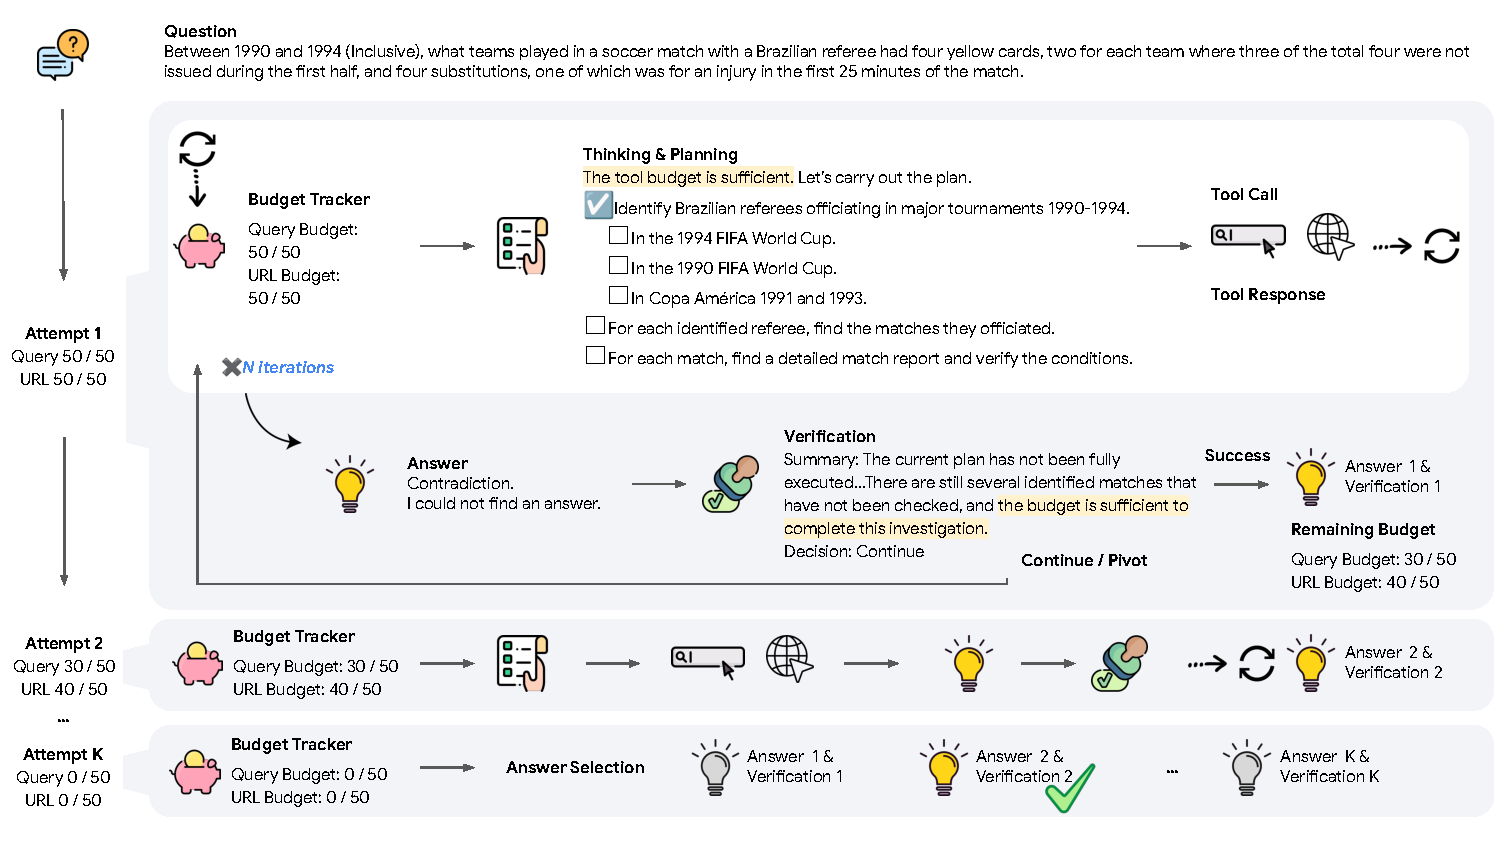
\includegraphics[width=\textwidth]{assets/figs/framework-bats.pdf} 
    \caption{Overview of the \method framework. Given a question and per-tool budgets, the agent begins with budget-aware thinking and planning, structured as a checklist. The agent keeps iterating by reasoning over new information and updated budgets. When an answer is proposed, \method performs verification and decides to either continue, pivot, or initiate a new attempt with the remaining budget. \method terminates when any of the budgets are exhausted.}
    \label{fig:framework}
\end{figure}

Given the demonstrated effectiveness of budget awareness, we now explore how it enhances agent orchestration and influences key behaviors such as planning and self-verification.
In this section, we propose \textbf{\method}, a \textbf{B}udget-\textbf{A}ware \textbf{T}est-time \textbf{S}caling framework for tool-augmented agents under explicit budget. As shown in Figure~\ref{fig:framework}, given an information-seeking question and a tool call budget, \method begins with internal reasoning to formulate a structured action plan and decide which tools to invoke.
Tool calls are triggered through specific tokens, and the returned tool responses are appended to the reasoning sequence, expanding the context with new evidence.  
When the agent proposes a candidate answer, the verification module checks its validity and decides whether to continue the current sequence or initiate a new attempt with the remaining budget. The iterative process terminates once any budgeted resource is exhausted. Finally, an LLM-as-a-judge selects the best answer across all verified answers. The full system instructions of \method are provided in Appendix~\ref{app:prompts}.


The central design principle of \method is \textit{budget awareness}. Throughout the execution, the Budget Tracker continuously updates both resource usage and remaining budget at every iteration.
This persistent awareness shapes the agent’s planning, tool-use strategy, and verification behavior, enabling adaptive and efficient use of constrained resources. We next describe how each module in \method incorporates budget awareness.




\subsection{Budget-Aware Planning}
% question decomposition and structured planning

Planning in \method incorporates both \emph{constraint decomposition} and \emph{structured dynamic planning}. 
Selecting an appropriate starting point is critical: a well-chosen entry narrows the search space and conserves budget, while a poor choice can quickly exhaust the budget (see example in Appendix~\ref{app:case_plan}).
To address this, we prompt the agent to first perform \textbf{constraint decomposition} and to categorize the clues implied in the question into two types: (1) \emph{exploration}, which expand the candidate space, and (2) \emph{verification}, which validate specific properties. While a verification clue can sometimes provide a direct shortcut to the answer, relying on it prematurely is risky, as it may consume resources without guaranteeing progress. 

The agent is further instructed to generate and maintain an explicit plan throughout execution. This \textbf{tree-structured plan} acts as a dynamic checklist, recording step status, resource usage, and allocation, while guiding future actions. It is never overwritten: completed, failed, or partial steps remain recorded to prevent redundant tool calls and to maintain a full execution trace. We provide the full prompt of planning module in Appendix~\ref{app:prompt_plan}.
As shown in the planning block from  Figure~\ref{fig:framework}, a single step in the plan represents a subtask that requires multiple tool calls to complete, for instance, getting a candidate list. 
After every iteration, new information may create additional branches, resolve pending steps, or invalidate unproductive paths. The planning module adjusts exploration breadth and verification depth based on the current remaining budget. 

This integration of constraint decomposition, persistent structured planning, and continuous budget-conditioned updating allows \method to maintain a controlled and interpretable search process while efficiently allocating available tool calls across exploration and verification subtasks. 




\subsection{Budget-Aware Self-verification}
% answer verification, decision, summary
Once the agent proposes an answer, the self-verification module re-evaluates the reasoning trajectory and corresponding resource usage. The full verifier prompt is provided in Appendix~\ref{app:prompt_verification}. This process begins with a constraint-by-constraint backward check. Using the previously extracted exploration and verification clues, the module assesses each constraint and determines whether it has been satisfied, contradicted, or remains unverifiable. This detailed check grounds the proposed answer directly against the question's requirements and clues. 


Based on this analysis, the module then makes a verification decision based on the above assessment and budget status. If all constraints are satisfied, the answer is marked as a \textit{SUCCESS}. If several constraints remain unverifiable but the trajectory appears promising, provided the budget is sufficient for deeper exploration, the outcome is to \textit{CONTINUE} exploration. In contrast, if contradictions are identified or the remaining budget cannot support further investigation towards this lead, the agent is expected to terminate expensive or low-yield directions early and \textit{PIVOT} toward a different direction to avoid wasting tool call resources while resources are still sufficient to pursue alternatives.

When the decision is to \textit{CONTINUE} or \textit{PIVOT}, the module also generates a concise summary that replaces the raw trajectory in context. This includes key reasoning steps, intermediate findings, failure causes, and suggestions for optimization to avoid redundant exploration.
By compressing the reasoning trajectory into a compact and informative summary, the verifier reduces context length while ensuring that subsequent attempts remain grounded in previously acquired information.

Together, structured constraint checking, explicit decision rules, and budget-aware trajectory summarization allow \method to terminate useless trajectories early, continue promising ones efficiently, and maintain reliable progress toward the correct answer within strict budget constraints. 
